\documentclass[10pt,a4paper]{article}

%double si on veut une version prof et une version élève. simple si on veut une seule version.
\newcommand{\buildmode}{simple}

\InputIfFileExists{version.tex}{}{}
% Version (définie par le script)
\providecommand{\version}{eleve}

\usepackage{feuilleinterro}

%%%à modifier à chaque fois

\renewcommand{\niveau}{1STMG}
\renewcommand{\chapitre}{Fonctions, généralités}
\renewcommand{\numchap}{0.1}
\renewcommand{\theme}{Fonctions}

%%%titre "CORRECTION" au lieu de "INTERROGATION", sans les champs Nom/Prénom
\renewcommand{\interroversion}[1]{
    \noindent\textbf{\niveau}

    \vspace{-0.5cm}
    \begin{center}
        \textbf{\large CORRECTION -- \chapitre}
    \end{center}

    \vspace{0.1cm}
}

\begin{document}

% =========================================================
% PAGE 1 : VERSION A
% =========================================================

\interroversion{A}

\textbf{Exercice 1 -- Tableau de valeurs \hfill /2}

On considère la fonction \(f\) définie sur \(\mathbb{R}\) par \(f(x)=x^2-2x-3\).

\[
\begin{aligned}
f(-2) &= (-2)^2-2\times(-2)-3 = 4+4-3 = 5\\
f(0)  &= 0^2-2\times 0-3 = 0-0-3 = -3
\end{aligned}
\]

\begin{center}
    \renewcommand{\arraystretch}{1.5}
    \setlength{\tabcolsep}{0.25cm}
    \begin{tabular}{|*{7}{c|}}
    \hline
    \(x\) & \(-2\) & \(-1\) & \(0\) & \(1\) & \(2\) & \(3\) \\
    \hline
    \(f(x)\) & \textcolor{blue}{\(5\)} & \(0\) & \textcolor{blue}{\(-3\)} & \(-4\) & \(-3\) & \(0\) \\
    \hline
    \end{tabular}
\end{center}

\textbf{Exercice 2 -- Lecture graphique \hfill /3}

On considère une fonction \(h\) dont la représentation graphique est donnée ci-dessous (ici \(h(x)=\frac{2}{3}(x-2)(x+1{,}5)(x-1)-1\)).

\begin{center}
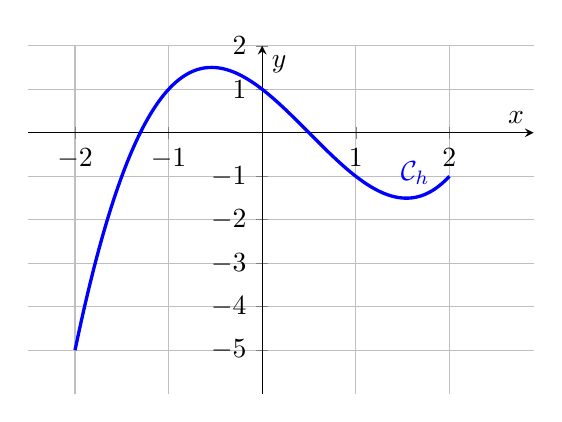
\begin{tikzpicture}
\begin{axis}[
    axis lines=middle,
    xmin=-2.5, xmax=2.9,
    ymin=-6, ymax=2,
    domain=-2:2,
    samples=300,
    grid=major,
    xtick={-2,-1,0,1,2,3},
    ytick={-5,-4,-3,-2,-1,0,1,2,3,4},
    xlabel={\(x\)},
    ylabel={\(y\)},
    width=8cm,
    height=6cm
]
\addplot[blue, very thick] {2/3*(x-2)*(x+1.5)*(x-1)-1}
node[pos=0.92, above right] {\(\mathcal{C}_h\)};
\end{axis}
\end{tikzpicture}
\end{center}

\begin{enumerate}
    \item Quel est l'ensemble de définition de \(h\) ? \hfill /1

    \(\mathcal{C}_h\) est tracée entre les abscisses \(-2\) et \(2\), donc \textcolor{blue}{\(D_h=[-2;2]\)}.
    \item Donner les images de \(-2\), \(0\) et \(1\) par \(h\). \hfill /1

    On lit l'ordonnée du point de \(\mathcal{C}_h\) d'abscisse \(-2\), puis \(0\), puis \(1\) :
    \textcolor{blue}{\(h(-2)=-5\), \(h(0)=1\), \(h(1)=-1\)}.
    \item Donner les éventuels antécédents de \(-1\) et de \(1\). \hfill /1

    \emph{Antécédents de \(-1\).} On lit les abscisses des points de \(\mathcal{C}_h\) d'ordonnée \(-1\) : \(x=-1{,}5\), \(x=1\) et \(x=2\).

    \emph{Antécédents de \(1\).} On lit les abscisses des points de \(\mathcal{C}_h\) d'ordonnée \(1\) : \(x=-1\) et \(x=0\).

    \textcolor{blue}{Antécédents de \(-1\) : \(-1{,}5\) ; \(1\) ; \(2\). Antécédents de \(1\) : \(-1\) ; \(0\).}
\end{enumerate}

\newpage

% =========================================================
% PAGE 2 : VERSION B
% =========================================================

\interroversion{B}

\textbf{Exercice 1 -- Tableau de valeurs \hfill /2}

On considère la fonction \(f\) définie sur \(\mathbb{R}\) par \(f(x)=x^2+x-2\).

\[
\begin{aligned}
f(-1) &= (-1)^2+(-1)-2 = 1-1-2 = -2\\
f(3)  &= 3^2+3-2 = 9+3-2 = 10
\end{aligned}
\]

\begin{center}
    \renewcommand{\arraystretch}{1.5}
    \setlength{\tabcolsep}{0.25cm}
    \begin{tabular}{|*{7}{c|}}
    \hline
    \(x\) & \(-2\) & \(-1\) & \(0\) & \(1\) & \(2\) & \(3\) \\
    \hline
    \(f(x)\) & \(0\) & \textcolor{blue}{\(-2\)} & \(-2\) & \(0\) & \(4\) & \textcolor{blue}{\(10\)} \\
    \hline
    \end{tabular}
\end{center}

\textbf{Exercice 2 -- Lecture graphique \hfill /3}

On considère une fonction \(h\) dont la représentation graphique est donnée ci-dessous (ici \(h(x)=\frac{2}{3}x(x+1)(x-2{,}5)-1\)).

\begin{center}
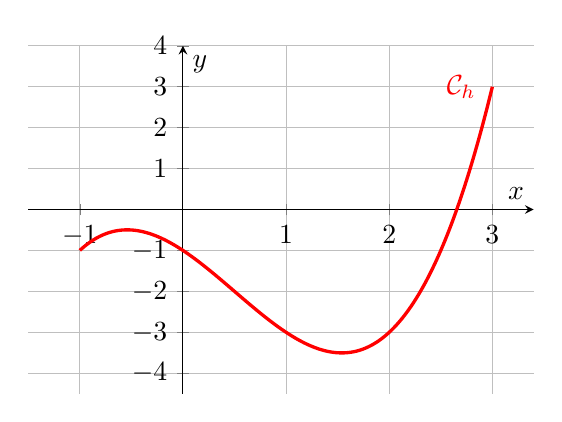
\begin{tikzpicture}
\begin{axis}[
    axis lines=middle,
    xmin=-1.5, xmax=3.4,
    ymin=-4.5, ymax=4,
    domain=-1:3,
    samples=300,
    grid=major,
    xtick={-2,-1,0,1,2,3,4},
    ytick={-4,-3,-2,-1,0,1,2,3,4},
    xlabel={\(x\)},
    ylabel={\(y\)},
    width=8cm,
    height=6cm
]
\addplot[red, very thick] {2/3*(x+1)*(x-2.5)*(x)-1}
node[pos=0.95, above left] {\(\mathcal{C}_h\)};
\end{axis}
\end{tikzpicture}
\end{center}

\begin{enumerate}
    \item Quel est l'ensemble de définition de \(h\) ? \hfill /1

    \(\mathcal{C}_h\) est tracée entre les abscisses \(-1\) et \(3\), donc \textcolor{blue}{\(D_h=[-1;3]\)}.
    \item Donner les images de \(-1\), \(0\) et \(2\) par \(h\). \hfill /1

    On lit l'ordonnée du point de \(\mathcal{C}_h\) d'abscisse \(-1\), puis \(0\), puis \(2\) :
    \textcolor{blue}{\(h(-1)=-1\), \(h(0)=-1\), \(h(2)=-3\)}.
    \item Donner les éventuels antécédents de \(-3\) et de \(-1\). \hfill /1

    \emph{Antécédents de \(-3\).} On lit les abscisses des points de \(\mathcal{C}_h\) d'ordonnée \(-3\) : \(x=1\) et \(x=2\).

    \emph{Antécédents de \(-1\).} On lit les abscisses des points de \(\mathcal{C}_h\) d'ordonnée \(-1\) : \(x=-1\), \(x=0\) et \(x=2{,}5\).

    \textcolor{blue}{Antécédents de \(-3\) : \(1\) ; \(2\). Antécédents de \(-1\) : \(-1\) ; \(0\) ; \(2{,}5\).}
\end{enumerate}

\newpage

% =========================================================
% PAGE 3 : VERSION C
% =========================================================

\interroversion{C}

\textbf{Exercice 1 -- Tableau de valeurs \hfill /2}

On considère la fonction \(f\) définie sur \(\mathbb{R}\) par \(f(x)=x^2-3x\).

\[
\begin{aligned}
f(-2) &= (-2)^2-3\times(-2) = 4+6 = 10\\
f(1)  &= 1^2-3\times 1 = 1-3 = -2
\end{aligned}
\]

\begin{center}
    \renewcommand{\arraystretch}{1.5}
    \setlength{\tabcolsep}{0.25cm}
    \begin{tabular}{|*{7}{c|}}
    \hline
    \(x\) & \(-2\) & \(-1\) & \(0\) & \(1\) & \(2\) & \(3\) \\
    \hline
    \(f(x)\) & \textcolor{blue}{\(10\)} & \(4\) & \(0\) & \textcolor{blue}{\(-2\)} & \(-2\) & \(0\) \\
    \hline
    \end{tabular}
\end{center}

\textbf{Exercice 2 -- Lecture graphique \hfill /3}

On considère une fonction \(h\) dont la représentation graphique est donnée ci-dessous (ici \(h(x)=\frac{1}{3}x(x+2)(x-2)-1\)).

\begin{center}
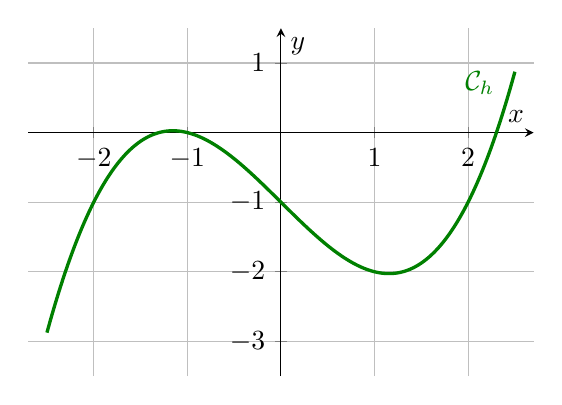
\begin{tikzpicture}
\begin{axis}[
    axis lines=middle,
    xmin=-2.7, xmax=2.7,
    ymin=-3.5, ymax=1.5,
    domain=-2.5:2.5,
    samples=300,
    grid=major,
    xtick={-2,-1,0,1,2},
    ytick={-3,-2,-1,0,1},
    xlabel={\(x\)},
    ylabel={\(y\)},
    width=8cm,
    height=6cm
]
\addplot[green!50!black, very thick] {1/3*(x+2)*x*(x-2)-1}
node[pos=0.95, above left] {\(\mathcal{C}_h\)};
\end{axis}
\end{tikzpicture}
\end{center}

\begin{enumerate}
    \item Quel est l'ensemble de définition de \(h\) ? \hfill /1

    \(\mathcal{C}_h\) est tracée entre les abscisses \(-2{,}5\) et \(2{,}5\), donc \textcolor{blue}{\(D_h=[-2{,}5;2{,}5]\)}.
    \item Donner les images de \(-2\), \(-1\) et \(1\) par \(h\). \hfill /1

    On lit l'ordonnée du point de \(\mathcal{C}_h\) d'abscisse \(-2\), puis \(-1\), puis \(1\) :
    \textcolor{blue}{\(h(-2)=-1\), \(h(-1)=0\), \(h(1)=-2\)}.
    \item Donner les éventuels antécédents de \(-1\) et de \(-2\). \hfill /1

    \emph{Antécédents de \(-1\).} On lit les abscisses des points de \(\mathcal{C}_h\) d'ordonnée \(-1\) : \(x=-2\), \(x=0\) et \(x=2\).

    \emph{Antécédents de \(-2\).} On lit les abscisses des points de \(\mathcal{C}_h\) d'ordonnée \(-2\) : \(x=1\), et deux autres valeurs, lues approximativement, proches de \(-2{,}3\) et de \(1{,}3\).

    \textcolor{blue}{Antécédents de \(-1\) : \(-2\) ; \(0\) ; \(2\). Antécédents de \(-2\) : \(1\) ; \(\approx-2{,}3\) ; \(\approx1{,}3\) (valeurs approchées, lues sur le graphique).}
\end{enumerate}

\newpage

% =========================================================
% PAGE 4 : VERSION D
% =========================================================

\interroversion{D}

\textbf{Exercice 1 -- Tableau de valeurs \hfill /2}

On considère la fonction \(f\) définie sur \(\mathbb{R}\) par \(f(x)=x^2+2x-1\).

\[
\begin{aligned}
f(-1) &= (-1)^2+2\times(-1)-1 = 1-2-1 = -2\\
f(2)  &= 2^2+2\times 2-1 = 4+4-1 = 7
\end{aligned}
\]

\begin{center}
    \renewcommand{\arraystretch}{1.5}
    \setlength{\tabcolsep}{0.25cm}
    \begin{tabular}{|*{7}{c|}}
    \hline
    \(x\) & \(-2\) & \(-1\) & \(0\) & \(1\) & \(2\) & \(3\) \\
    \hline
    \(f(x)\) & \(-1\) & \textcolor{blue}{\(-2\)} & \(-1\) & \(2\) & \textcolor{blue}{\(7\)} & \(14\) \\
    \hline
    \end{tabular}
\end{center}

\textbf{Exercice 2 -- Lecture graphique \hfill /3}

On considère une fonction \(h\) dont la représentation graphique est donnée ci-dessous (ici \(h(x)=\frac{1}{3}(x+2)(x+1)(x-3)\)).

\begin{center}
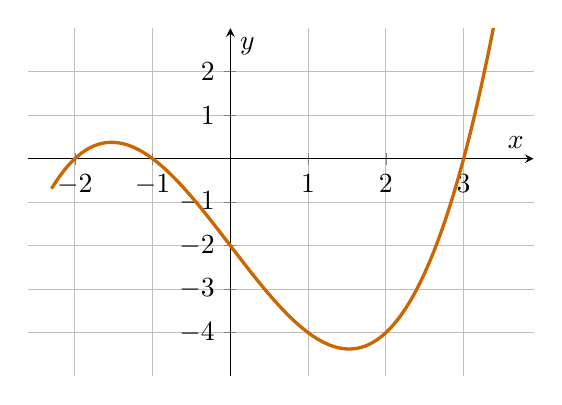
\begin{tikzpicture}
\begin{axis}[
    axis lines=middle,
    xmin=-2.6, xmax=3.9,
    ymin=-5, ymax=3,
    domain=-2.3:3.5,
    samples=300,
    grid=major,
    xtick={-2,-1,0,1,2,3},
    ytick={-4,-3,-2,-1,0,1,2},
    xlabel={\(x\)},
    ylabel={\(y\)},
    width=8cm,
    height=6cm
]
\addplot[orange!80!black, very thick] {1/3*(x+2)*(x+1)*(x-3)}
node[pos=0.95, above left] {\(\mathcal{C}_h\)};
\end{axis}
\end{tikzpicture}
\end{center}

\begin{enumerate}
    \item Quel est l'ensemble de définition de \(h\) ? \hfill /1

    \(\mathcal{C}_h\) est tracée entre les abscisses \(-2{,}3\) et \(3{,}5\), donc \textcolor{blue}{\(D_h=[-2{,}3;3{,}5]\)}.
    \item Donner les images de \(-2\), \(0\) et \(2\) par \(h\). \hfill /1

    On lit l'ordonnée du point de \(\mathcal{C}_h\) d'abscisse \(-2\), puis \(0\), puis \(2\) :
    \textcolor{blue}{\(h(-2)=0\), \(h(0)=-2\), \(h(2)=-4\)}.
    \item Donner les éventuels antécédents de \(0\) et de \(-4\). \hfill /1

    \emph{Antécédents de \(0\).} On lit les abscisses des points de \(\mathcal{C}_h\) d'ordonnée \(0\) : \(x=-2\), \(x=-1\) et \(x=3\).

    \emph{Antécédents de \(-4\).} On lit les abscisses des points de \(\mathcal{C}_h\) d'ordonnée \(-4\) : \(x=1\) et \(x=2\).

    \textcolor{blue}{Antécédents de \(0\) : \(-2\) ; \(-1\) ; \(3\). Antécédents de \(-4\) : \(1\) ; \(2\).}
\end{enumerate}

\end{document}
